\documentclass[12pt]{article}
 \usepackage[hcentering,bindingoffset=20mm]{geometry}
 \usepackage{placeins}
 \usepackage[numbib]{tocbibind}
 \usepackage{rotating}
\usepackage[square,sort,comma,numbers]{natbib}
 \usepackage{graphicx}
 \usepackage{tabularx}
 \linespread{1.3}
 \usepackage{gensymb}
\usepackage{longtable}
 \usepackage{lscape}
 \usepackage{url}
 \addtolength{\textwidth}{2cm}
 \addtolength{\hoffset}{-1cm}
 
 
 \addtolength{\textheight}{2cm}
 \addtolength{\voffset}{-1cm}
 \setlength{\parindent}{0pt}
 
\title{Using transcriptomics to investigate evolution and toxicology in \textit{Gambierdiscus}. $^{1}$}
\author{Key words: \emph{Gambierdiscus}, ciguatoxin, pan-transcriptome}
\date{}

\begin{document}
\maketitle
\paragraph{}Anna Liza Kretzschmar$^{2}$\\
Climate Change Cluster (C3), University of Technology Sydney, Ultimo, 2007 NSW, Australia, anna.kretzschmar@uts.edu.au
\paragraph{}Tim Kahlke\\
Climate Change Cluster (C3), University of Technology Sydney, Ultimo, 2007 NSW, Australia
\paragraph{}Kirsty Smith \\
Cawthron Institute, The Wood, Nelson 7010, New Zealanda
\paragraph{}Lesley Rhodes \\
Cawthron Institute, The Wood, Nelson 7010, New Zealand
\paragraph{}Aaron E. Darling \\
The ithree institute, University of Technology Sydney, Ultimo, 2007 NSW, Australia
\paragraph{}Shauna Murray\\ 
Climate Change Cluster (C3), University of Technology Sydney, Ultimo, 2007 NSW, Australia
\newpage
\section*{Abstract}
Species of the genus \textit{Gambierdiscus} produce Ciguatoxins (CTXs), the causative agent of ciguatera fish poisoning, a potentially debilitating seafood borne illness. 
Species of \textit{Gambierdiscus} possess very large genomes, 32 - 35 Gbp, and, as with other dinoflagellates, possess unique genomic characteristics, such as highly repetitive and complex genome architecture. 
The exact toxins produced by species of \textit{Gambierdiscus} remain largely unclear. 
It has been verified using LCMS on multiple strains that the species \textit{Gambierdiscus polynesiensis} produces anaologs of CTXs. 
Other species appear to produce maitotoxins, gambierol, and other uncharacterised toxins. 
An understanding of the evolution of \textit{Gambierdiscus} and their toxins requires information regarding their genetics. 
Transcriptomic sequencing is a feasible alternative to genome sequencing. 
In this study, we generated de novo RNA-seq libraries for \textit{Gambierdiscus polynesiensis}, \textit{Gambierdiscus carpenteri}, \textit{Gambierdiscus} cf. \textit{silvae} and \textit{Gambierdiscus lapillus}, compared these to a previously sequenced \textit{Gambierdiscus australes}, to discover a set of core genes shared by all species. 
We present a Gambierdiscus core transcriptome, which might be used to investigate candidate genes related to toxin production.\\
Further to investigate CTX production more specifically, we compared two CTX -producing strains of \textit{Gambierdiscus polynesiensis} to one non-CTX producing strain, verified by LC-MS/MS, to look for clues about pathways involved in ciguatoxin production.

\newpage
\section*{Introduction}
%more shit for manuscript:
%- Gambierdiscus intro, clinical relevance of CFP, interest in monitoring\\
%-protist genome sizes, obstacles with sequencing, lack of reference genomes available \\
%- transcriptomes as alternative, dino genetic elements, transcriptomes a good stand in for ref genome\\
%- G. polynesiensis and implications in CFP specifically, CTX and associated search for PKS genes\\
%- focus of study: core-transcriptome for \textit{Gambierdiscus} for RNA-seq reference purposes and polynesiensis comparison to look for expression differences between toxic and non-toxic strains

%chapter intro stuff:
\subsection*{general dino stuff, genetic peculiarities}
 - loss of nucleosomes \cite{rizzo1972chromosomal}\\
- high DNA content \cite{lajeunesse2005symbiodinium}\\
- thymine nucleotide replacement with uracil \cite{rae1976hydroxymethyluracil}\\
- plastic and mitochondrial genes widely incorporated into - genome \cite{bachvaroff2004dinoflagellate}\\
- horizontal gene transfer rife\\
- potential unlinking of transciptome and observed protein expression \cite{bachvaroff2008stop}\\
- large gene families \\
- trans-splicing creates pool of fully mature, useable mRNA that can then be selected from .. may be why transcriptome good approximation of genome \cite{lidie2007spliced,zhang2007spliced}\\
- werid as fuck transcription factors \cite{guillebault2002new}\\
- dinoSL .. trans-spliced leader present in 2/3 of genes detected and in 12/15 of highly expressed \cite{bachvaroff2008stop,lidie2007spliced}\\
- genes of highly expressed proteins are present in tandem arrays \cite{bachvaroff2008stop}\\
- post-transcriptional control of protein expression and extremely long mRNA half lives \cite{morey2013global}\\
- smRNA as possible post-transcriptional regulation mechanism \cite{baumgarten2013integrating}

\subsection*{importance of ref genome}
The analysis of any genetic data relies on the reference to a known, closely related entity. 
Without a functional protein or genome reference database, the generation of sequencing data would be like pissing in the wind. 
A reference is essential in determining both the adequacy of the sequencing methodology as well as interpretation of results. 
           

\subsection*{due to no ref gen, importance of transciptome and features that allow for approximation}

\subsection*{other pan-tran work ie koid and bacterial.. yeast?}

\subsection*{In this study.. go through LC-MS and toxicology info}

\newpage
\section*{Methods}
%more shit for manuscript:
%\subsection*{Culture conditions}
% Kirsty to insert method but not in chapter
%\subsection*{RNA isolation}
% Kirsty to insert method but not in chapter
%\subsection*{Library prep and sequencing}
% Kirsty to insert method but not in chapter
Scripts used for this project are available on Github under hydrahamster/pan-tran.
\subsection*{Transcriptome acquisition}
Transcriptomes used in this chapter were the RNA-seq libraries for \textit{G. carpenteri} (UTSMER9A3), \textit{G. lapillus} (HG4), \textit{G. polynesiensis} (CG15) and \textit{G.} cf. \textit{silvae} (HG5) generated for \textbf{chapter 4}. 
\textit{G. australes} (CAWD149) RNA-seq library was downloaded from the MMETSP public database. 
Seq libraries were assembled as per the transcriptome assembly subsection in the methods of \textit{chapter 4}, without diginorm. 


\subsection*{Homolog clustering}
Cd-hit was used to cluster the contigs from assemblies with the flags T 10 -M 5000 -G 0 -c 1.00 -aS 1.00 -aL 0.005 \cite{fu2012cd}. 
Then Transdecoder predicted the protein coding regions of the nucleotide clusters which were subsequently clustered adain with cd-hit as before with the exception of -c 0.98 \cite{haas2016transdecoder}.
Protein clusters were annotated with Interproscan v5.27 with local lookup server \cite{quevillon2005interproscan}.
Protein clusters were processed to include the species of origin instead of the TRINITY tag and concatenated for input to get\_homologues \cite{vinuesa2015robust}. 
The -t 0 flag was used for get\_homologues to acquire all possible clusters even with only one species representative, and -G for the OMCL algorithm. 
The resulting pan-, core- and softcore-clusters were matched with their interpro annotations and GO terms were queried with GOSUM \textbf{-- Tim how do I cit this?}. 
GOSUM was run at both levels 1 and 2 of gene ontology counts with the go-basic gene ontology version. 

\subsection*{PKS search}
The transcriptome assemblies were queried for the five conserved PKS active domains using hmmer \cite{eddy2015hmmer} with libraries developed for this project. 
The identified contigs for an active domain was then searched for within the clusters to identify how the active domains grouped together between species.

%\subsection*{\textit{G. polynesiensis} comparison}
\newpage
\section*{Results}
\FloatBarrier
%\subsection*{Transcriptome overview}
%- seq and annotation stats for \textit{Gambierdiscus polynesiensis} CAWD254 and Table ~\ref{tbl:SeqTable}
\subsection*{General info}
The progression of clustering and annotation results per transcriptome can be found in ~\ref{tbl:ClustTable}.
\begin{table}
\caption{Progression of clusters found in each \emph{Gambierdiscus} transcriptome during processing.}
\label{tbl:ClustTable}
\begin{tabular}{ | p{3cm} | p{2cm} | p{2.5cm} | p{2.5cm} | p{2cm} | p{2cm}|}
\hline
\textbf{Species}& \textit{G. australes} (CAWD149)& \emph{G. carpenteri} (UTSMER9A3)&\emph{G. lapillus} (HG4)&\emph{G. polynesiensis} (CG15)&\emph{G.} cf. \emph{silvae} (HG5)\\
\hline
\textbf{Contigs}&&263,829&148,972&270,315&191,224\\
\hline
\textbf{Nucleotide clusters}&102,861&263,743&148,966&270,265&191,205\\
\hline
\textbf{Predicted coding regions}&63,299&180,568&111,862&176,290&132,688\\
\hline
\textbf{Protein clusters}&60,166&139,699&92,418&139,487&107,766\\
\hline
%\hline
%&&&&&\\
\end{tabular}
\end{table}
\FloatBarrier
\newpage

\subsection*{\emph{Gambierdiscus} inter-species core-transcriptome}
- number of clusters\\
- percentage annotated \\
- highest number of contigs per cluster and what pathway\\
- heatmap if I can get it working
- annotation differences between transcriptomes
\begin{figure} 
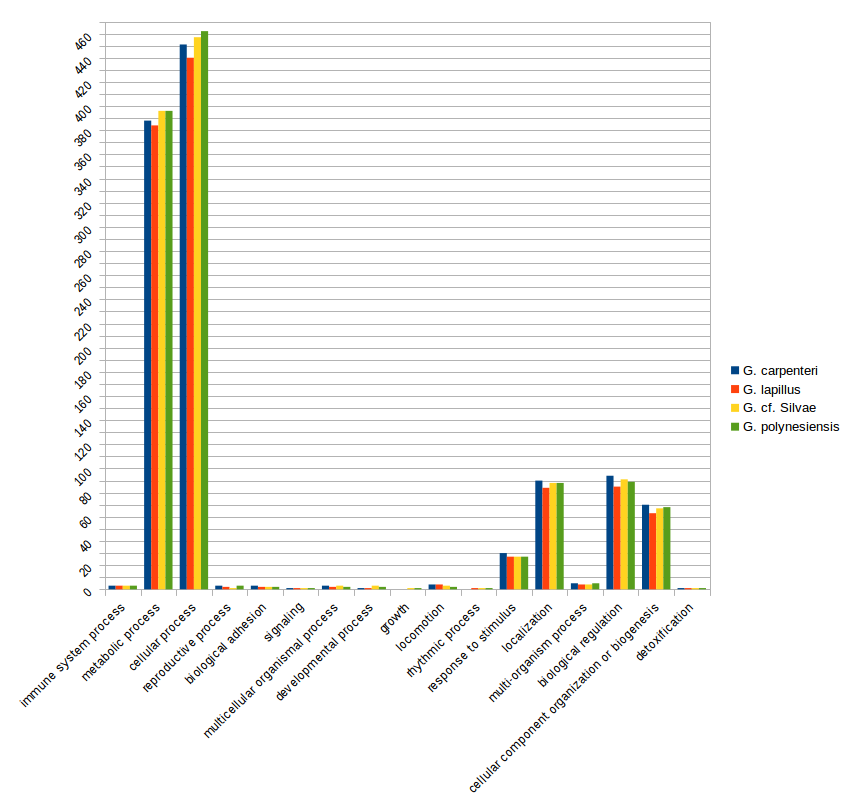
\includegraphics[scale=.78]{3Aug18_cluster-investigation/figures/gosum-species/Species-gosum1-bio.png} 
\caption{Summary of biological processes GO annotations between core, softcore and unique clusters at GOSUM level 1.} 
\label{fig:SpecGo1Bio}
\end{figure} 
\FloatBarrier

\begin{figure} 
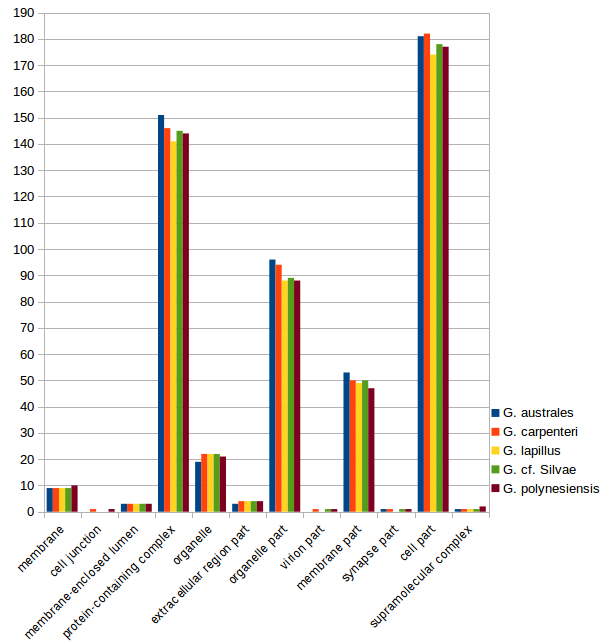
\includegraphics[scale=.8]{3Aug18_cluster-investigation/figures/gosum-species/Species-gosum1-cell.png} 
\caption{Summary of cellular GO annotations between core, softcore and unique clusters at GOSUM level 1.} 
\label{fig:SpecGo1Cell}
\end{figure} 
\FloatBarrier

\begin{figure} 
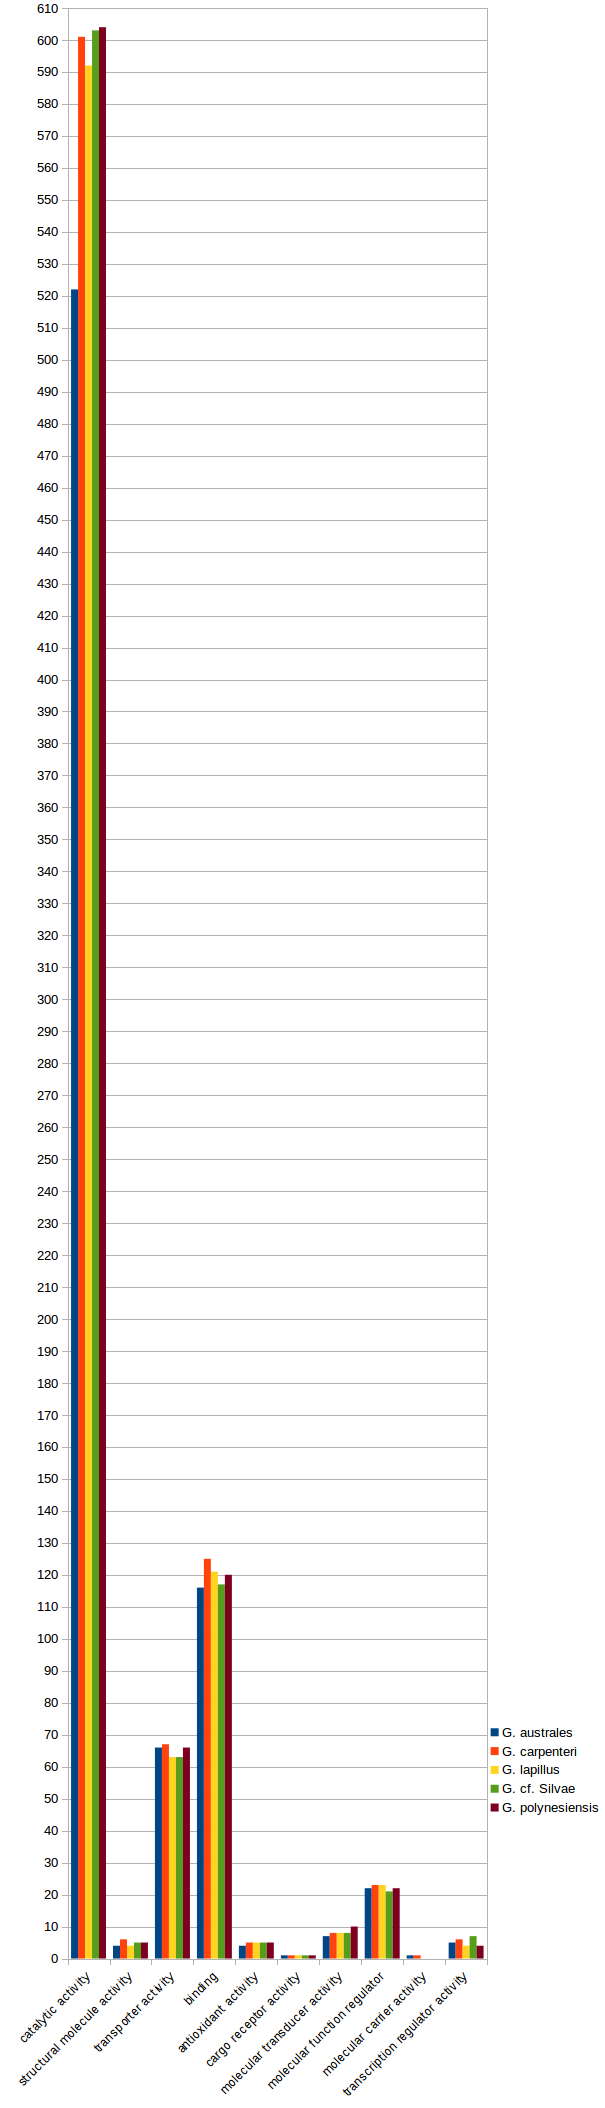
\includegraphics[scale=1]{3Aug18_cluster-investigation/figures/gosum-species/Species-gosum1-molec.png} 
\caption{Summary of molecular GO annotations between core, softcore and unique clusters at GOSUM level 1.} 
\label{fig:SpecGo1Molec}
\end{figure} 
\FloatBarrier

\begin{figure} 
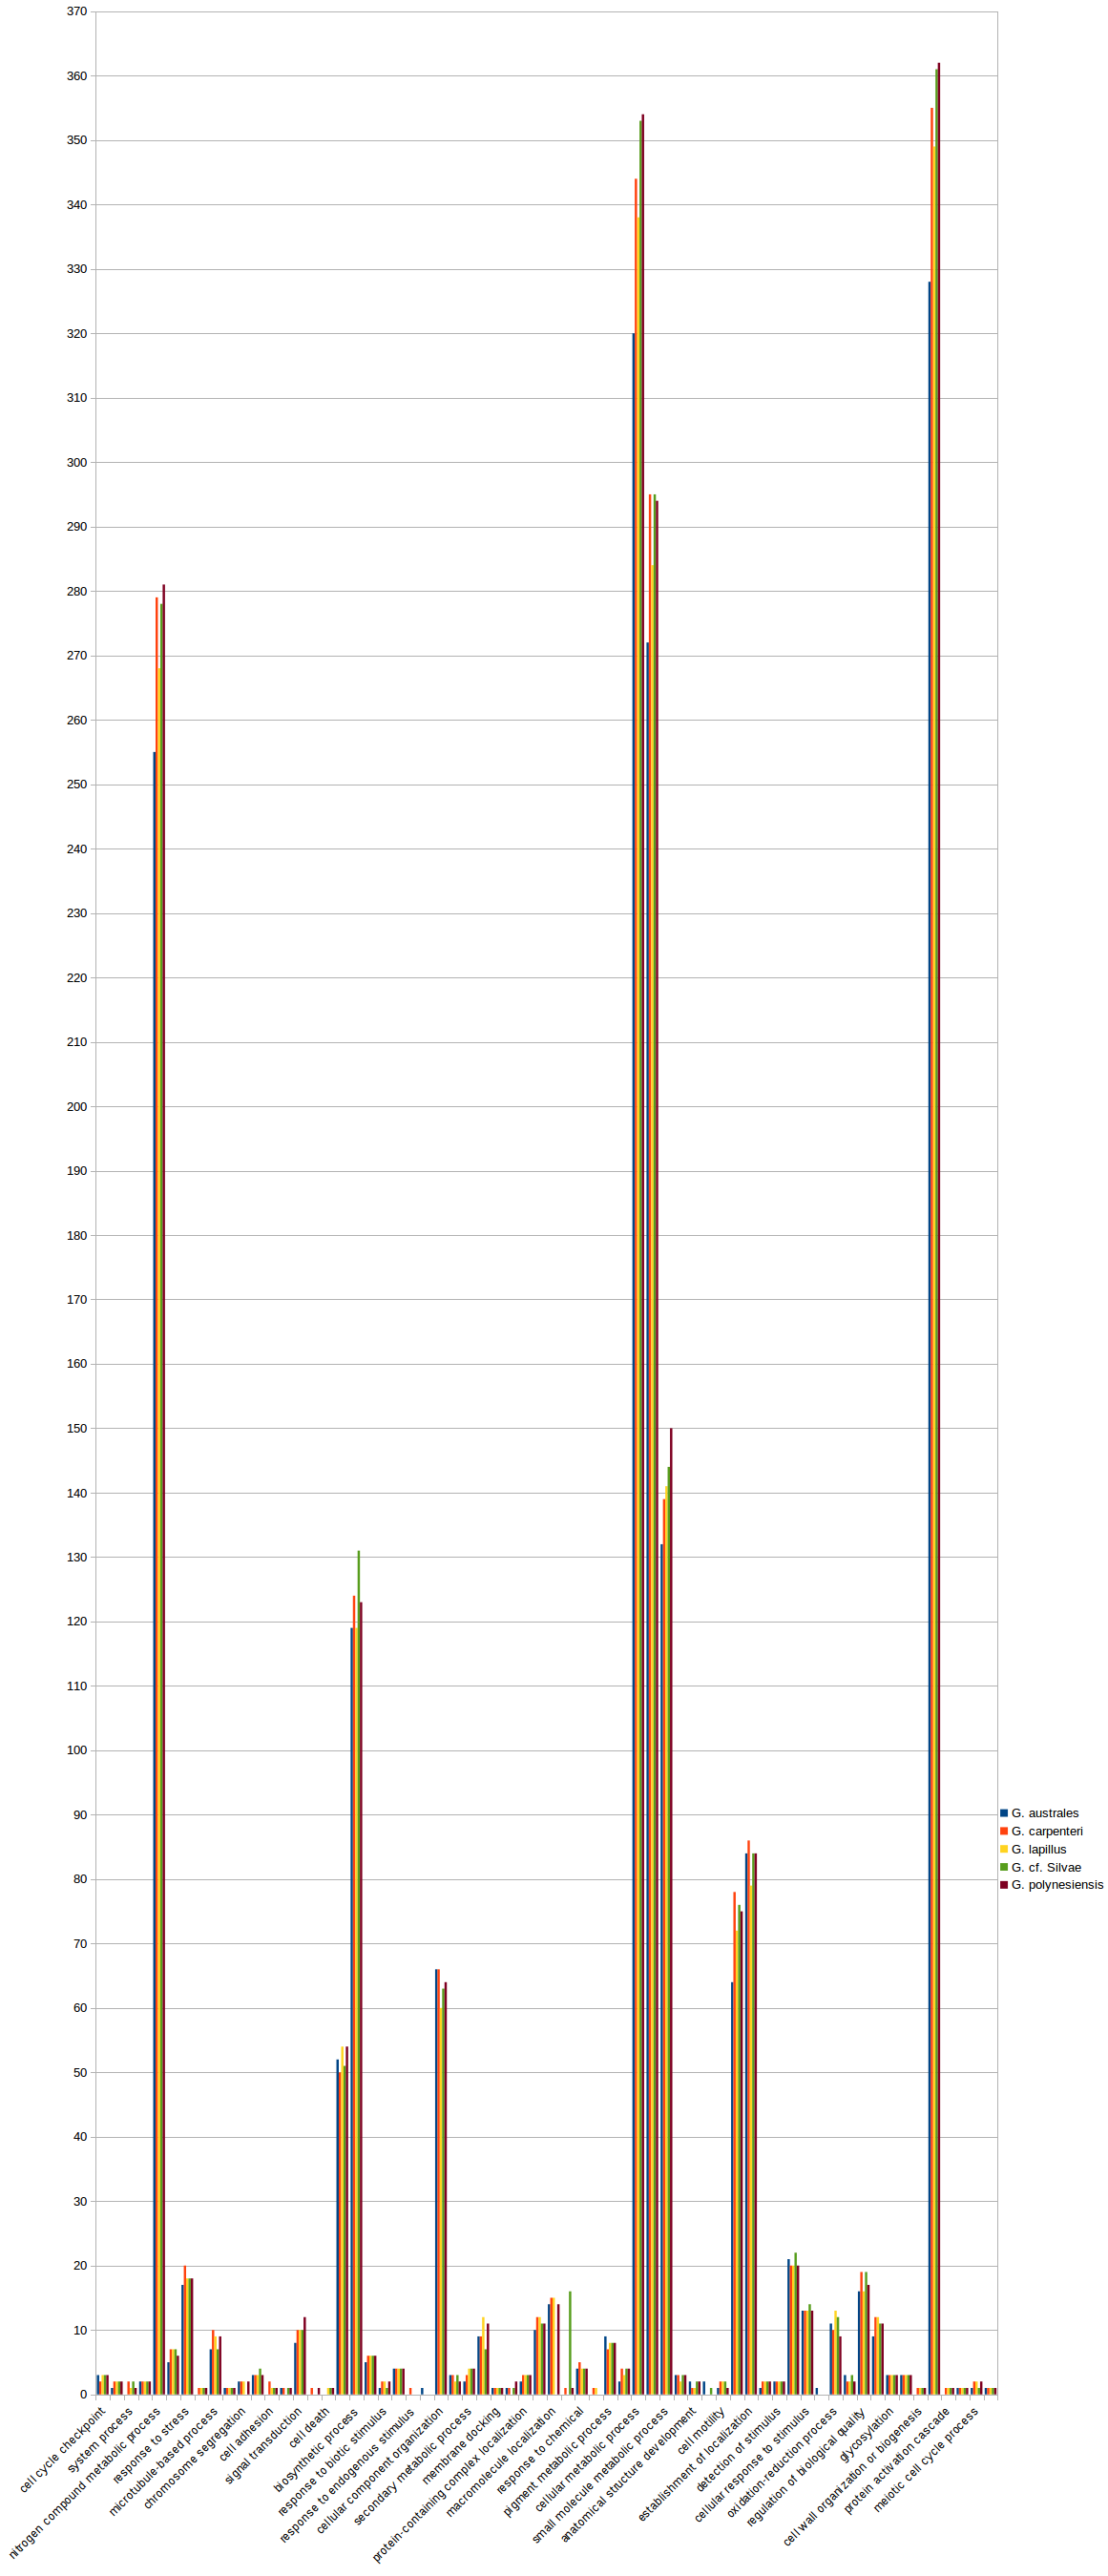
\includegraphics[scale=.9]{3Aug18_cluster-investigation/figures/gosum-species/Species-gosum2-bio.png} 
\caption{Summary of biological processes GO annotations between core, softcore and unique clusters at GOSUM level 2.} 
\label{fig:SpecGo2Bio}
\end{figure} 
\FloatBarrier

\begin{figure} 
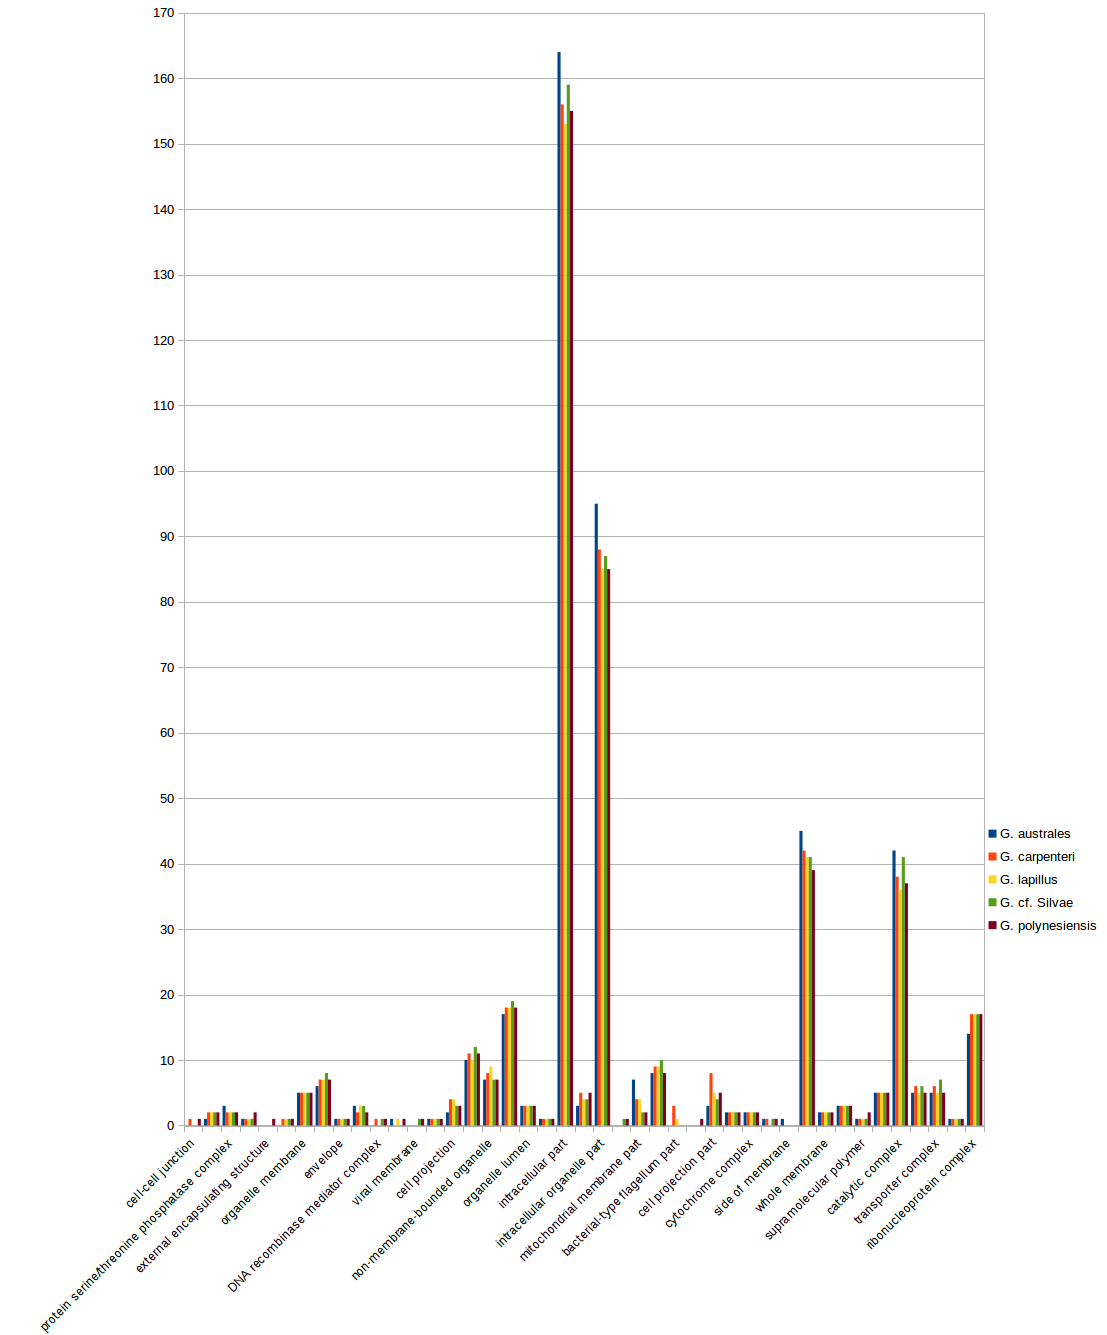
\includegraphics[scale=1]{3Aug18_cluster-investigation/figures/gosum-species/Species-gosum2-cell.png} 
\caption{Summary of cellular GO annotations between core, softcore and unique clusters at GOSUM level 2.} 
\label{fig:SpecGo2Cell}
\end{figure} 
\FloatBarrier

\begin{figure} 
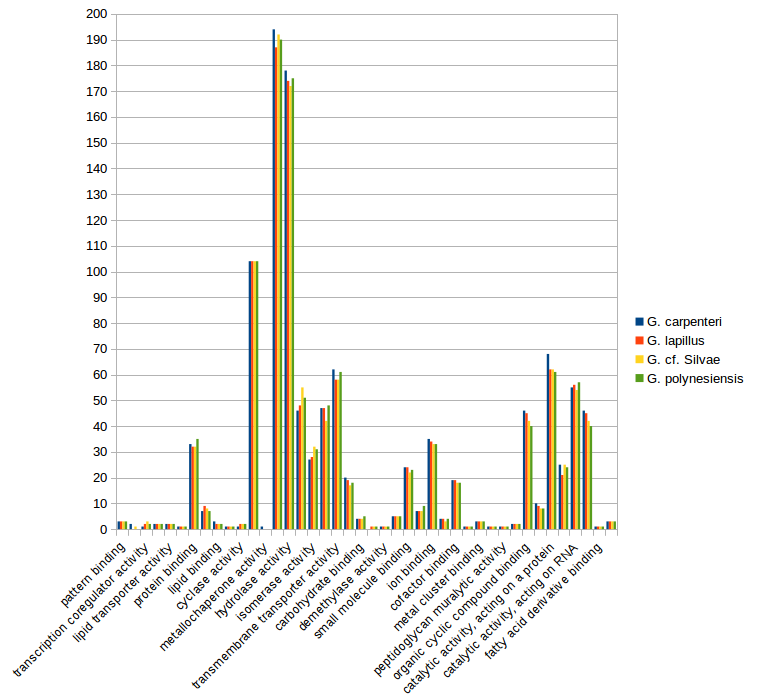
\includegraphics[scale=.85]{3Aug18_cluster-investigation/figures/gosum-species/Species-gosum2-molec.png} 
\caption{Summary of molecular GO annotations between core, softcore and unique clusters at GOSUM level 2.} 
\label{fig:SpecGo2Molec}
\end{figure} 
\FloatBarrier

\subsubsection*{Core transcritome}
- number of clusters\\
- percentage annotated \\
- GOSUM summary \\
- pathways present
\subsubsection*{Softcore - 4 of 5 species}
- number of clusters\\
- percentage annotated \\
- pathways present\\
- which most commonly not present
\subsection*{\emph{Gambierdiscus} inter-species pan-transcriptome}
- which species most commonly solo\\
- number of clusters\\
- percentage annotated \\
- pathways present\\
- any change in contig numbers between species within clusters
\subsubsection*{Unique clusters}
- which species most commonly solo\\
- number of clusters\\
- percentage annotated \\
- pathways present\\


%\subsection*{\emph{Gambierdiscus polynesiensis} intra-species core \& pan transcriptome}
\subsection*{Looking into toxin producers}
\subsubsection*{Clusters with \textit{G. lapillus}, \textit{G. polynesiensis} \& \textit{G. cf. silvae}}
\subsubsection*{\textit{G. polynesiensis solo clusters}}
- number of clusters\\
- percentage annotated \\
- pathways present\\
\subsubsection*{Polyketide synthase genes}
- number of contigs found in each transcriptome\\
- how many clusters do they end up in and what is the proportion of species in there \\
- any multi-domain ones?\\

\begin{table}
\caption{\emph{Gambierdiscus} species transcriptomes used in this study along with their toxicity, toxin profile, accession numbers and source.}
\label{tbl:SeqTable}
\begin{tabular}{ | p{3cm} | p{2cm} | p{2.5cm} | p{2.5cm} | p{2cm} | p{2cm}|}
\hline
\textbf{Species} & \textbf{Source location}&\textbf{LC-MS/MS} & \textbf{Toxicity via bioassay} & \textbf{Accession ID} & \textbf{References} \\
\hline
\textit{Gambierdiscus australes} (CAWD149)&Rarotonga, Cook Islands& CTX -ve; MTX +ve&CTX +ve; MTX N/A&MMETSP0766&\cite{keeling2014marine,rhodes2010toxic,rhodes2014production,munday2017ciguatoxins}\\
\hline
\textit{Gambierdiscus carpenteri} (UTSMER9A)&Merimbula, NSW, Australia&CTX -ve; MTX -ve&CTX -ve; MTX +ve&SRR6821720
&\textbf{chapter 4} \& \cite{larsson2018toxicology}\\
\hline
\textit{Gambierdiscus lapillus} (HG4)&Heron Island, QLD, Australia&CTX -ve; MTX +ve&CTX +ve; MTX +ve&SRR6821722
&\textbf{chapter 4} \& \cite{larsson2018toxicology,kretzschmar2017characterization}\\
\hline
\textit{Gambierdiscus polynesiensis} (CG15)&Rarotonga, Cook Islands&CTX +ve; MTX +ve&CTX N/A; MTX N/A&SRR6821723
&\textbf{chapter 4} \\
\hline
%\textit{Gambierdiscus polynesiensis}&CAWD212&CTX +ve; MTX +ve&CTX N/A; MTX N/A&Kohli pers. comm.&\cite{rhodes2014production}\\
%\hline
%\textit{Gambierdiscus polynesiensis}&CAWD254&CTX -ve; MTX -ve&CTX N/A; MTX N/A&&This study\\
%\hline
\textit{Gambierdiscus} cf. \textit{silvae} (HG5)&Heron Island, QLD, Australia&CTX -ve; MTX +ve&CTX +ve; MTX +ve&SRR6821721
&\textbf{chapter 4} \& \cite{larsson2018toxicology,kretzschmar2017characterization}\\
\hline
\end{tabular}
\end{table}
\FloatBarrier
\newpage
\section*{Discussion}
-overall summary of study

\subsection*{core \textit{Gambierdiscus} transcriptome}
- \cite{lidie2005gene} comprehensive index of genes in K. brevis to compare to 

\subsubsection*{discuss common \& different gene pathways found}

\begin{figure} 
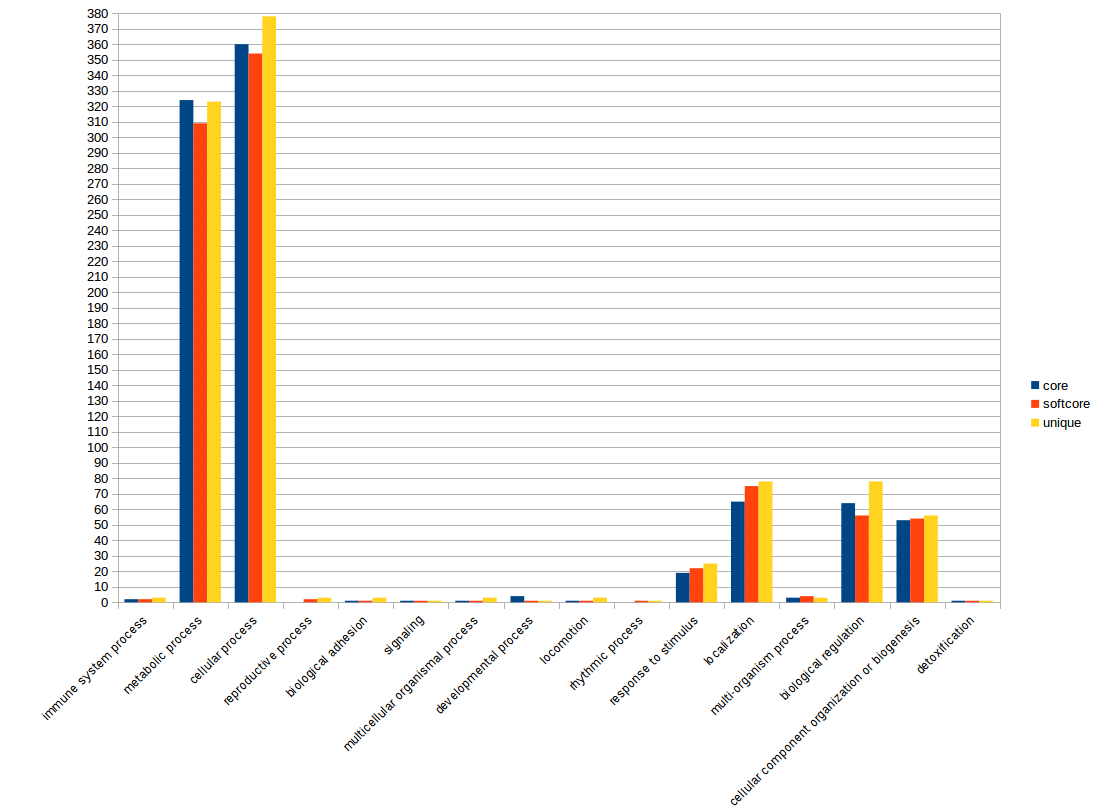
\includegraphics[scale=.6]{3Aug18_cluster-investigation/figures/gosum-pan/Pan-gosum1-bio-graph.png} 
\caption{Summary of biological processes GO annotations between core, softcore and unique clusters at GOSUM level 1.} 
\label{fig:PanGo1Bio}
\end{figure} 
\FloatBarrier

\begin{figure} 
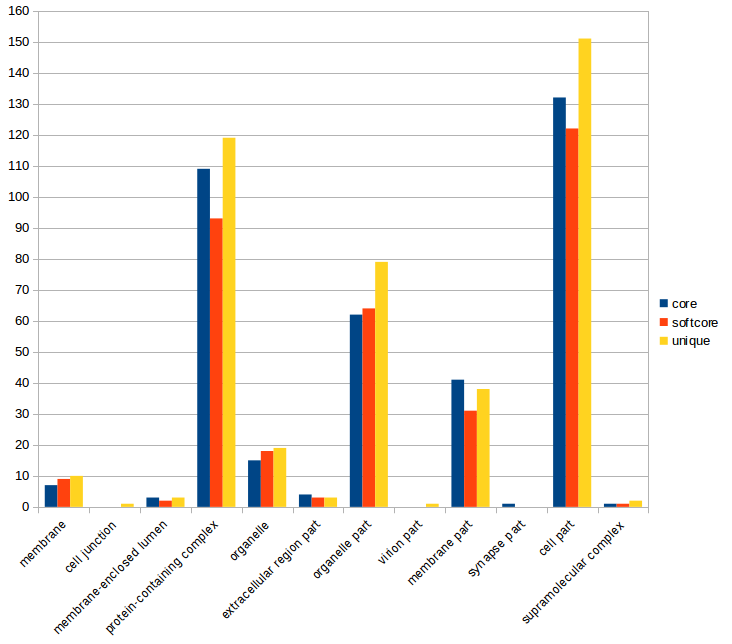
\includegraphics[scale=.8]{3Aug18_cluster-investigation/figures/gosum-pan/Pan-gosum1-cell-graph.png} 
\caption{Summary of cellular GO annotations between core, softcore and unique clusters at GOSUM level 1.} 
\label{fig:PanGo1Cell}
\end{figure} 
\FloatBarrier

\begin{figure} 
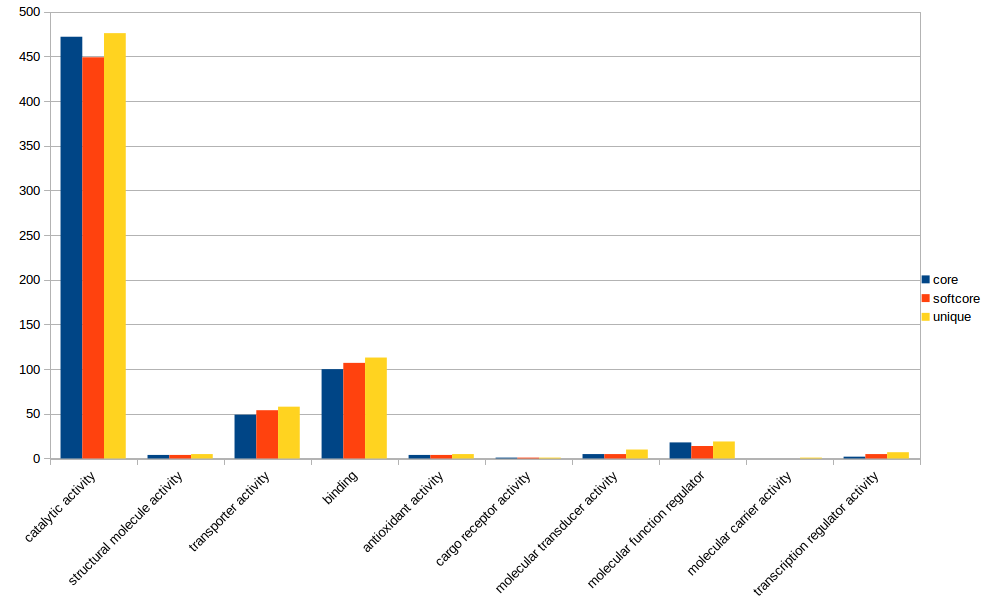
\includegraphics[scale=.65]{3Aug18_cluster-investigation/figures/gosum-pan/Pan-gosum1-molec-graph.png} 
\caption{Summary of molecular GO annotations between core, softcore and unique clusters at GOSUM level 1.} 
\label{fig:PanGo1Molec}
\end{figure} 
\FloatBarrier

\begin{figure} 
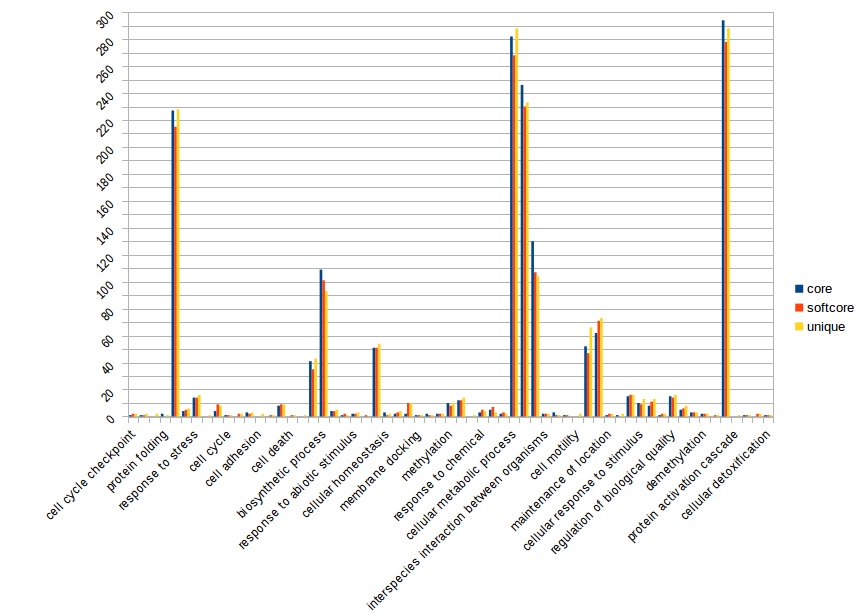
\includegraphics[scale=.75]{3Aug18_cluster-investigation/figures/gosum-pan/Pan-gosum2-bio-graph.png} 
\caption{Summary of biological processes GO annotations between core, softcore and unique clusters at GOSUM level 2.} 
\label{fig:PanGo2Bio}
\end{figure} 
\FloatBarrier

\begin{figure} 
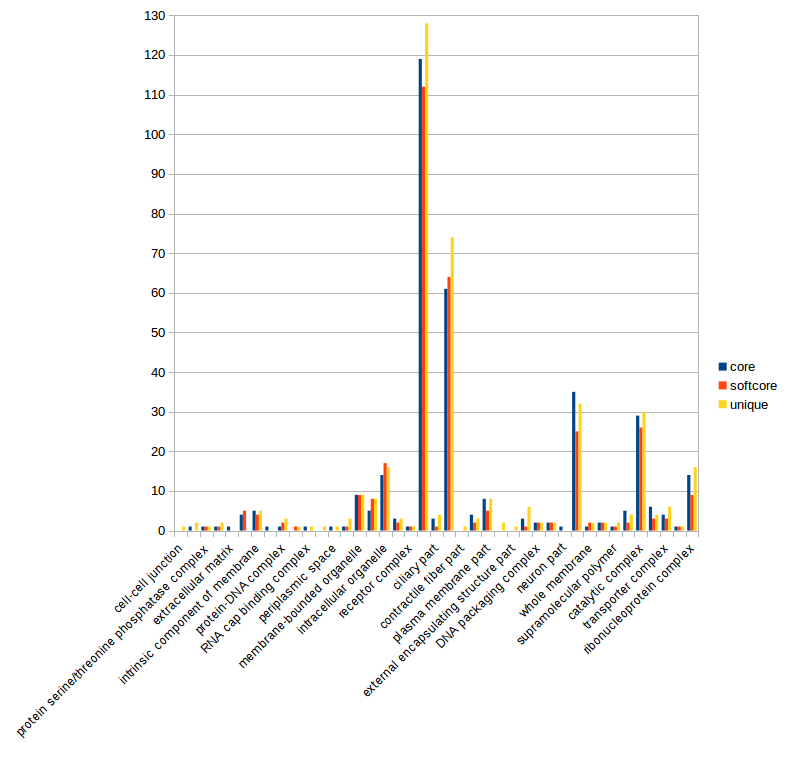
\includegraphics[scale=.8]{3Aug18_cluster-investigation/figures/gosum-pan/Pan-gosum2-cell-graph.png} 
\caption{Summary of cellular GO annotations between core, softcore and unique clusters at GOSUM level 2.} 
\label{fig:PanGo2Cell}
\end{figure} 
\FloatBarrier

\begin{figure} 
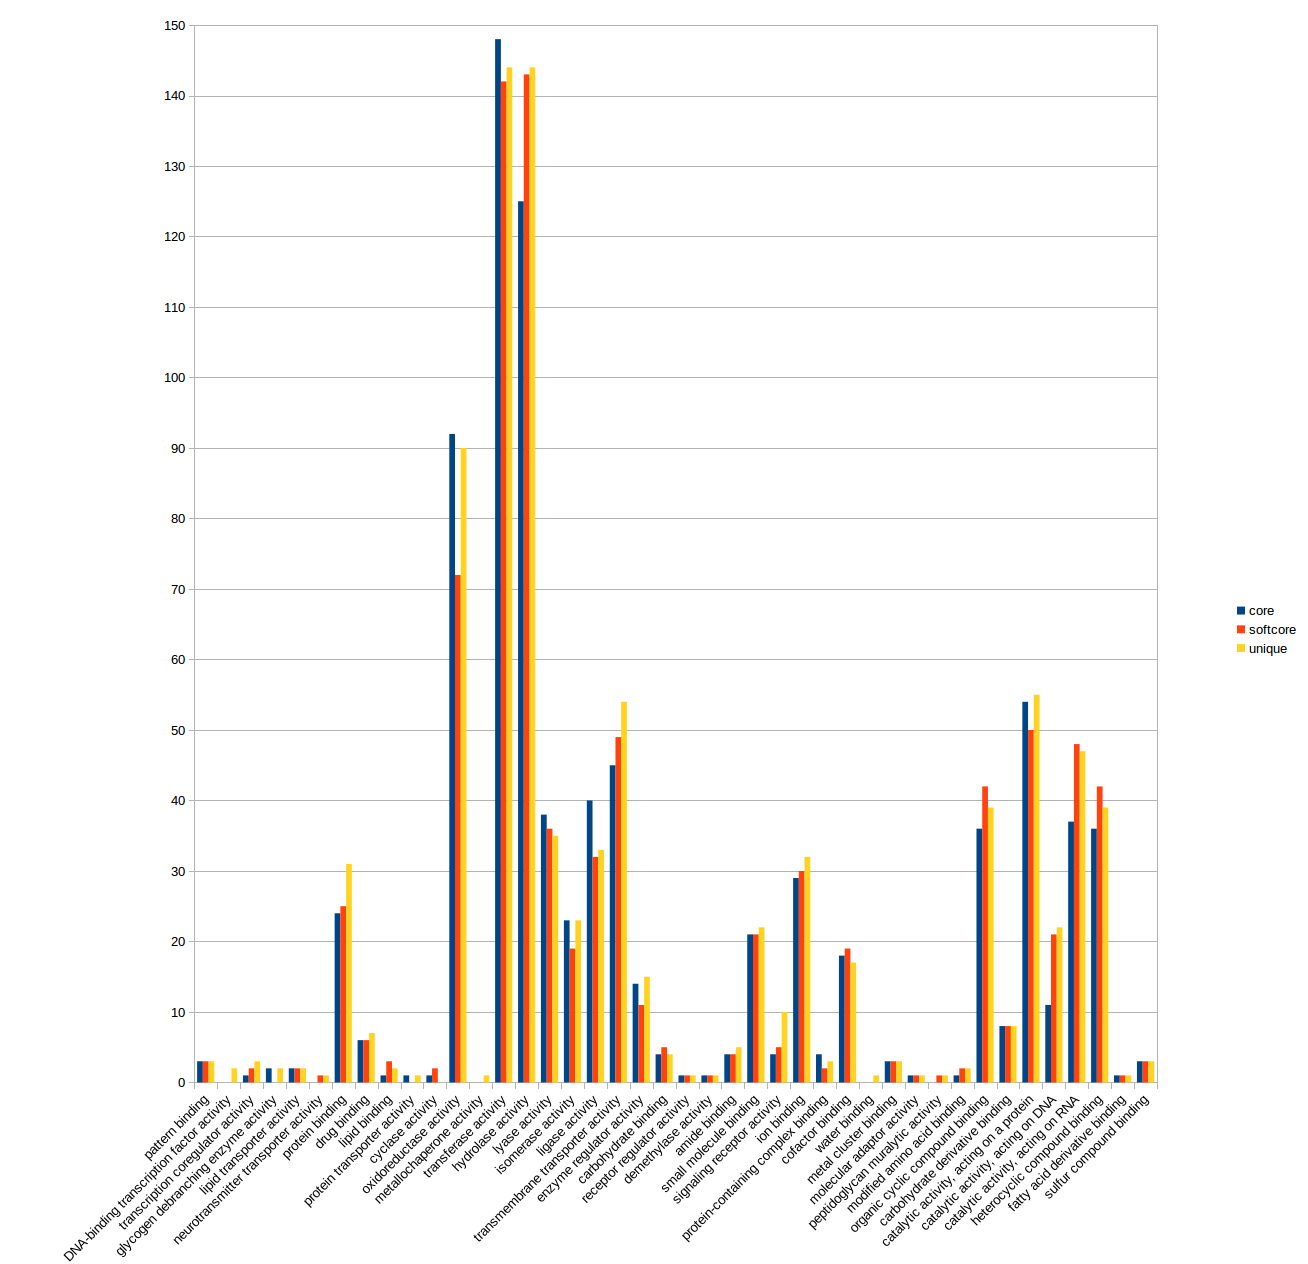
\includegraphics[scale=.6]{3Aug18_cluster-investigation/figures/gosum-pan/Pan-gosum2-molec-graph.png} 
\caption{Summary of molecular GO annotations between core, softcore and unique clusters at GOSUM level 2.} 
\label{fig:PanGo2Molec}
\end{figure} 
\FloatBarrier

\subsubsection*{discuss usefulness for future studies}

\subsubsection*{Expression of genes involved in polyketide production}
- discuss if different gene sets were expressed between toxic and non- toxic strains\\
- discuss if diff genes between all 3 strains\\
- discuss short comings with CAWD254 not having bioassays run, sequencing differences etc

\subsubsection*{discuss potential short commings} 
- from different seq runs and methods and seq depth may vary, especially \textit{G. australes} \\
- intra-speces variation so one isolate per species may not be representative \\
- unknown if processes other than PKS play a role in toxin production
%\subsection*{core \textit{G. polynesiensis} transcriptome}
%- discuss common gene pathways found \\
%-discuss usefulness for future studies\\
%-discuss potential short commings

%\newpage
\section*{Conclusion}


\section*{Supplementary}
- gosum tables with GO annotations

\FloatBarrier
\begin{longtable}{ | p{2.2cm} | p{4cm} |p{2cm} | p{2cm} | p{2cm} | p{2cm} |}
\caption{GO terms and number of contigs per species at GO ontology level 1.}\\
\hline
\label{tbl:SpGO1}
GO acession&GO terms&\emph{G. carpenteri}&\emph{G. lapillus}&\emph{G. polynesiensis}&\emph{G.} cf. \emph{silvae}\\
\hline
 \multicolumn{6}{| c |}{Biological processes}\\
 \hline
GO:0002376&immune system process&3&3&3&3\\
 \hline
GO:0008152&metabolic process&388&384&396&396\\
 \hline
GO:0009987&cellular process&451&440&457&462\\
 \hline
GO:0022414&reproductive process&3&2&1&3\\
 \hline
GO:0022610&biological adhesion&3&2&2&2\\
 \hline
GO:0023052&signaling&1&1&1&1\\
 \hline
GO:0032501&multicellular organismal process&3&2&3&2\\
 \hline
GO:0032502&developmental process&1&1&3&2\\
 \hline
GO:0040007&growth&0&0&1&1\\
 \hline
GO:0040011&locomotion&4&4&3&2\\
 \hline
GO:0048511&rhythmic process&0&1&1&1\\
 \hline
GO:0050896&response to stimulus&30&27&27&27\\
 \hline
GO:0051179&localization&90&84&88&88\\
 \hline
GO:0051704&multi-organism process&5&4&4&5\\
 \hline
GO:0065007&biological regulation&94&85&91&89\\
 \hline
GO:0071840&cellular component organization/biogenesis&70&63&67&68\\
 \hline
GO:0098754&detoxification&1&1&1&1\\
\hline
 \multicolumn{6}{| c |}{Cellular components}\\
 \hline
GO:0016020&membrane&9&9&9&10\\
 \hline
GO:0030054&cell junction&1&0&0&1\\
 \hline
GO:0031974&membrane-enclosed lumen&3&3&3&3\\
 \hline
GO:0032991&protein-containing complex&146&141&145&144\\
 \hline
GO:0043226&organelle&22&22&22&21\\
 \hline
GO:0044421&extracellular region part&4&4&4&4\\
 \hline
GO:0044422&organelle part&94&88&89&88\\
 \hline
GO:0044423&virion part&1&0&1&1\\
 \hline
GO:0044425&membrane part&50&49&50&47\\
 \hline
GO:0044456&synapse part&1&0&1&1\\
 \hline
GO:0044464&cell part&182&174&178&177\\
 \hline
GO:0099080&supramolecular complex&1&1&1&2\\
\hline
 \multicolumn{6}{| c |}{Molecular function}\\
\hline
GO:0003824&catalytic activity&601&592&603&604\\
\hline
GO:0005198&structural molecule activity&6&4&5&5\\
\hline
GO:0005215&transporter activity&67&63&63&66\\
\hline
GO:0005488&binding&125&121&117&120\\
\hline
GO:0016209&antioxidant activity&5&5&5&5\\
\hline
GO:0038024&cargo receptor activity&1&1&1&1\\
\hline
GO:0060089&molecular transducer activity&8&8&8&10\\
\hline
GO:0098772&molecular function regulator&23&23&21&22\\
\hline
GO:0140104&molecular carrier activity&1&0&0&0\\
\hline
GO:0140110&transcription regulator activity&6&4&7&4\\
\hline
\end{longtable}

\FloatBarrier
\begin{longtable}{ | p{2.2cm} | p{4cm} |p{2cm} | p{2cm} | p{2cm} | p{2cm} |}
\caption{GO terms and number of contigs per species at GO ontology level 2, child terms of Table ~\ref{tbl:SpGO1}.}\\
\hline
\label{tbl:SpGO2}
GO acession&GO terms&\emph{G. carpenteri}&\emph{G. lapillus}&\emph{G. polynesiensis}&\emph{G.} cf. \emph{silvae}\\
\hline
 \multicolumn{6}{| c |}{Biological processes}\\
 \hline
GO:0000075&cell cycle checkpoint&2&3&3&3\\
 \hline
GO:0002252&immune effector process&2&2&2&2\\
 \hline
GO:0003008&system process&2&1&2&1\\
 \hline
GO:0006457&protein folding&2&2&2&2\\
 \hline
GO:0006807&nitrogen compound metabolic process&279&268&278&281\\
 \hline
GO:0006928&movement of cell or subcellular component&7&7&7&6\\
 \hline
GO:0006950&response to stress&20&18&18&18\\
 \hline
GO:0006955&immune response&1&1&1&1\\
 \hline
GO:0007017&microtubule-based process&10&9&7&9\\
 \hline
GO:0007049&cell cycle&1&1&1&1\\
 \hline
GO:0007059&chromosome segregation&2&2&0&2\\
 \hline
GO:0007154&cell communication&3&3&4&3\\
 \hline
GO:0007155&cell adhesion&2&1&1&1\\
 \hline
GO:0007163&establishment or maintenance of cell polarity&1&0&1&1\\
 \hline
GO:0007165&signal transduction&10&10&10&12\\
 \hline
GO:0008037&cell recognition&1&0&0&1\\
 \hline
GO:0008219&cell death&0&1&1&1\\
 \hline
GO:0009056&catabolic process&50&54&51&54\\
 \hline
GO:0009058&biosynthetic process&124&119&131&123\\
 \hline
GO:0009605&response to external stimulus&6&6&6&6\\
 \hline
GO:0009607&response to biotic stimulus&2&2&1&2\\
 \hline
GO:0009628&response to abiotic stimulus&4&4&4&4\\
 \hline
GO:0009719&response to endogenous stimulus&1&0&0&0\\
 \hline
GO:0016043&cellular component organization&66&60&63&64\\
 \hline
GO:0019725&cellular homeostasis&3&2&3&2\\
 \hline
GO:0019748&secondary metabolic process&3&4&4&4\\
 \hline
GO:0022402&cell cycle process&9&12&7&11\\
 \hline
GO:0022406&membrane docking&1&1&1&1\\
 \hline
GO:0030029&actin filament-based process&1&0&1&2\\
 \hline
GO:0031503&protein-containing complex localization&3&3&3&3\\
 \hline
GO:0032259&methylation&12&12&11&11\\
 \hline
GO:0033036&macromolecule localization&15&15&0&14\\
 \hline
GO:0035036&sperm-egg recognition&1&0&16&1\\
 \hline
GO:0042221&response to chemical&5&4&4&4\\
 \hline
GO:0042330&taxis&1&1&0&0\\
 \hline
GO:0042440&pigment metabolic process&7&8&8&8\\
 \hline
GO:0044085&cellular component biogenesis&4&3&4&4\\
 \hline
GO:0044237&cellular metabolic process&344&338&353&354\\
 \hline
GO:0044238&primary metabolic process&295&284&295&294\\
 \hline
GO:0044281&small molecule metabolic process&139&141&144&150\\
 \hline
GO:0044419&interspecies interaction between organisms&3&2&3&3\\
 \hline
GO:0048856&anatomical structure development&1&1&2&2\\
 \hline
GO:0048869&cellular developmental process&0&0&1&\\
 \hline
GO:0048870&cell motility&2&2&2&1\\
 \hline
GO:0050789&regulation of biological process&78&72&76&75\\
 \hline
GO:0051234&establishment of localization&86&79&84&84\\
 \hline
GO:0051235&maintenance of location&2&2&2&2\\
 \hline
GO:0051606&detection of stimulus&2&2&2&2\\
 \hline
GO:0051641&cellular localization&20&20&22&20\\
 \hline
GO:0051716&cellular response to stimulus&13&13&14&13\\
 \hline
GO:0055114&oxidation-reduction process&10&13&12&9\\
 \hline
GO:0061919&process utilizing autophagic mechanism&2&2&3&2\\
 \hline
GO:0065008&regulation of biological quality&19&16&19&17\\
 \hline
GO:0065009&regulation of molecular function&12&12&11&11\\
 \hline
GO:0070085&glycosylation&3&3&3&3\\
 \hline
GO:0070988&demethylation&3&3&3&3\\

GO:0071554&cell wall organization or biogenesis&1&1&1&1\\

GO:0071704&organic substance metabolic process&355&349&361&362\\
 \hline
GO:0072376&protein activation cascade&1&1&1&1\\
 \hline
GO:0140029&exocytic process&1&1&1&1\\
 \hline
GO:1903046&meiotic cell cycle process&2&2&1&2\\
 \hline
GO:1990748&cellular detoxification&1&1&1&1\\
\hline
 \multicolumn{6}{| c |}{Cellular components}\\
 \hline
GO:0005911&cell-cell junction&1&0&0&1\\
 \hline
GO:0005929&cilium&2&2&2&2\\
 \hline
GO:0008287&protein serine/threonine phosphatase complex&2&2&2&2\\
 \hline
GO:0019867&outer membrane&1&1&1&2\\
 \hline
GO:0030312&external encapsulating structure&0&0&0&1\\
 \hline
GO:0031012&extracellular matrix&1&1&1&1\\
 \hline
GO:0031090&organelle membrane&5&5&5&5\\
 \hline
GO:0031224&intrinsic component of membrane&7&7&8&7\\
 \hline
GO:0031975&envelope&1&1&1&1\\
 \hline
GO:0032993&protein-DNA complex&2&3&3&2\\
 \hline
GO:0033061&DNA recombinase mediator complex&1&0&1&1\\
 \hline
GO:0034518&RNA cap binding complex&0&1&0&1\\
 \hline
GO:0036338&viral membrane&0&0&1&1\\
 \hline
GO:0042597&periplasmic space&1&1&1&1\\
 \hline
GO:0042995&cell projection&4&4&3&3\\
 \hline
GO:0043227&membrane-bounded organelle&11&10&12&11\\
 \hline
GO:0043228&non-membrane-bounded organelle&8&9&7&7\\
 \hline
GO:0043229&intracellular organelle&18&18&19&18\\
 \hline
GO:0043233&organelle lumen&3&3&3&3\\
 \hline
GO:0043235&receptor complex&1&1&1&1\\
 \hline
GO:0044424&intracellular part&156&153&159&155\\
 \hline
GO:0044441&ciliary part&5&4&4&5\\
 \hline
GO:0044446&intracellular organelle part&88&85&87&85\\
 \hline
GO:0044449&contractile fiber part&0&0&1&1\\
 \hline
GO:0044455&mitochondrial membrane part&4&4&2&2\\
 \hline
GO:0044459&plasma membrane part&9&9&10&8\\
 \hline
GO:0044461&bacterial-type flagellum part&3&1&0&0\\
 \hline
GO:0044462&external encapsulating structure part&0&0&0&1\\
 \hline
GO:0044463&cell projection part&8&5&4&5\\
 \hline
GO:0044815&DNA packaging complex&2&2&2&2\\
 \hline
GO:0070069&cytochrome complex&2&2&2&2\\
 \hline
GO:0097458&neuron part&1&0&1&1\\
 \hline
GO:0098796&membrane protein complex&42&41&41&39\\
 \hline
GO:0098805&whole membrane&2&2&2&2\\
 \hline
GO:0099023&tethering complex&3&3&3&3\\
 \hline
GO:0099081&supramolecular polymer&1&1&1&2\\
 \hline
GO:0120114&Sm-like protein family complex&5&5&5&5\\
 \hline
GO:1902494&catalytic complex&38&36&41&37\\
 \hline
GO:1990204&oxidoreductase complex&6&5&6&5\\
 \hline
GO:1990351&transporter complex&6&5&7&5\\
 \hline
GO:1990391&DNA repair complex&1&1&1&1\\
 \hline
GO:1990904&ribonucleoprotein complex&17&17&17&17\\
\hline
 \multicolumn{6}{| c |}{Molecular function}\\
\hline
GO:0001871&pattern binding&3&3&3&3\\
\hline
GO:0003700&DNA-binding transcription factor activity&2&0&1&0\\
\hline
GO:0003712&transcription coregulator activity&1&2&3&2\\
\hline
GO:0004133&glycogen debranching enzyme activity&2&2&2&2\\
\hline
GO:0005319&lipid transporter activity&2&2&2&2\\
\hline
GO:0005326&neurotransmitter transporter activity&1&1&1&1\\
\hline
GO:0005515&protein binding&33&32&32&35\\
\hline
GO:0008144&drug binding&7&9&8&7\\
\hline
GO:0008289&lipid binding&3&2&2&2\\
\hline
GO:0008565&protein transporter activity&1&1&1&1\\
\hline
GO:0009975&cyclase activity&1&2&2&2\\
\hline
GO:0016491&oxidoreductase activity&104&104&104&104\\
\hline
GO:0016530&metallochaperone activity&1&0&0&0\\
\hline
GO:0016740&transferase activity&194&187&192&190\\
\hline
GO:0016787&hydrolase activity&178&174&172&175\\
\hline
GO:0016829&lyase activity&46&48&55&51\\
\hline
GO:0016853&isomerase activity&27&28&32&31\\
\hline
GO:0016874&ligase activity&47&47&42&48\\
\hline
GO:0022857&transmembrane transporter activity&62&58&58&61\\
\hline
GO:0030234&enzyme regulator activity&20&19&17&18\\
\hline
GO:0030246&carbohydrate binding&4&4&4&5\\
\hline
GO:0030545&receptor regulator activity&0&1&1&1\\
\hline
GO:0032451&demethylase activity&1&1&1&1\\
\hline
GO:0033218&amide binding&5&5&5&5\\
\hline
GO:0036094&small molecule binding&24&24&22&23\\
\hline
GO:0038023&signaling receptor activity&7&7&7&9\\
\hline
GO:0043167&ion binding&35&34&33&33\\
\hline
GO:0044877&protein-containing complex binding&4&4&3&4\\
\hline
GO:0048037&cofactor binding&19&19&18&18\\
\hline
GO:0050824&water binding&1&1&1&1\\
\hline
GO:0051540&metal cluster binding&3&3&3&3\\
\hline
GO:0060090&molecular adaptor activity&1&1&1&1\\
\hline
GO:0061783&peptidoglycan muralytic activity&1&1&1&1\\
\hline
GO:0072341&modified amino acid binding&2&2&2&2\\
\hline
GO:0097159&organic cyclic compound binding&46&45&42&40\\
\hline
GO:0097367&carbohydrate derivative binding&10&9&8&8\\
\hline
GO:0140096&catalytic activity, acting on a protein&68&62&62&61\\
\hline
GO:0140097&catalytic activity, acting on DNA&25&21&25&24\\
\hline
GO:0140098&catalytic activity, acting on RNA&55&56&54&57\\
\hline
GO:1901363&heterocyclic compound binding&46&45&42&40\\
\hline
GO:1901567&fatty acid derivative binding&1&1&1&1\\
\hline
GO:1901681&sulfur compound binding&3&3&3&3\\
\hline
\end{longtable}


\FloatBarrier
\begin{longtable}{ | p{2.2cm} | p{4cm} |p{2cm} | p{2cm} | p{2cm} | }
\caption{GO terms and number of contigs found in core, softcore and pan-transcriptome of \textit{Gambierdiscus} at GO ontology level 1.}\\
\hline
\label{tbl:PanGO1}
GO acession&GO terms&Core&Softcore&Pan\\
\hline
 \multicolumn{5}{| c |}{Biological processes}\\
 \hline
GO:0002376&immune system process&2&2&3\\
 \hline
GO:0008152&metabolic process&324&309&323\\
 \hline
GO:0009987&cellular process&360&354&378\\
 \hline
GO:0022414&reproductive process&0&2&3\\
 \hline
GO:0022610&biological adhesion&1&1&3\\
 \hline
GO:0023052&signaling&1&1&1\\
 \hline
GO:0032501&multicellular organismal process&1&1&3\\
 \hline
GO:0032502&developmental process&4&1&1\\
 \hline
GO:0040011&locomotion&1&1&3\\
 \hline
GO:0048511&rhythmic process&0&1&1\\
 \hline
GO:0050896&response to stimulus&19&22&25\\
 \hline
GO:0051179&localization&65&75&78\\
 \hline
GO:0051704&multi-organism process&3&4&3\\
 \hline
GO:0065007&biological regulation&64&56&78\\
 \hline
GO:0071840&cellular component organization or biogenesis&53&54&56\\
 \hline
GO:0098754&detoxification&1&1&1\\
\hline
 \multicolumn{5}{| c |}{Cellular components}\\
 \hline
GO:0016020&membrane&7&9&10\\ 
 \hline 
GO:0030054&cell junction&0&0&1\\ 
 \hline 
GO:0031974&membrane-enclosed lumen&3&2&3\\ 
 \hline 
GO:0032991&protein-containing complex&109&93&119\\ 
 \hline 
GO:0043226&organelle&15&18&19\\ 
 \hline 
GO:0044421&extracellular region part&4&3&3\\ 
 \hline 
GO:0044422&organelle part&62&64&79\\ 
 \hline 
GO:0044423&virion part&0&0&1\\ 
 \hline 
GO:0044425&membrane part&41&31&38\\ 
 \hline 
GO:0044456&synapse part&1&0&0\\ 
 \hline 
GO:0044464&cell part&132&122&151\\ 
 \hline 
GO:0099080&supramolecular complex&1&1&2\\ 
\hline
 \multicolumn{5}{| c |}{Molecular function}\\
\hline
GO:0003824&catalytic activity&472&449&476\\ 
 \hline 
GO:0005198&structural molecule activity&4&4&5\\ 
 \hline 
GO:0005215&transporter activity&49&54&58\\ 
 \hline 
GO:0005488&binding&100&107&113\\ 
 \hline 
GO:0016209&antioxidant activity&4&4&5\\ 
 \hline 
GO:0038024&cargo receptor activity&1&1&1\\ 
 \hline 
GO:0060089&molecular transducer activity&5&5&10\\ 
 \hline 
GO:0098772&molecular function regulator&18&14&19\\ 
 \hline 
GO:0140104&molecular carrier activity&0&0&1\\ 
 \hline 
GO:0140110&transcription regulator activity&2&5&7\\ 
\hline
\end{longtable}

\FloatBarrier
\begin{longtable}{ | p{2.2cm} | p{4cm} |p{2cm} | p{2cm} | p{2cm} | }
\caption{GO terms and number of contigs found in core, softcore and pan-transcriptome of \textit{Gambierdiscus} at GO ontology level 2, childer to Table ~\ref{tbl:PanGO1}.}\\
\hline
\label{tbl:PanGO2}
GO acession&GO terms&Core&Softcore&Pan\\
\hline
 \multicolumn{5}{| c |}{Biological processes}\\
 \hline
GO:0000075&cell cycle checkpoint&1&2&2\\ 
 \hline 
GO:0002252&immune effector process&1&1&2\\ 
 \hline 
GO:0003008&system process&0&0&2\\ 
 \hline 
GO:0006457&protein folding&2&0&1\\ 
 \hline 
GO:0006807&nitrogen compound metabolic process&227&215&228\\ 
 \hline 
GO:0006928&movement of cell or subcellular component&4&5&6\\ 
 \hline 
GO:0006950&response to stress&14&14&16\\ 
 \hline 
GO:0006955&immune response&0&0&1\\ 
 \hline 
GO:0007017&microtubule-based process&4&9&8\\ 
 \hline 
GO:0007049&cell cycle&1&1&1\\ 
 \hline 
GO:0007059&chromosome segregation&0&2&2\\ 
 \hline 
GO:0007154&cell communication&3&2&3\\ 
 \hline 
GO:0007155&cell adhesion&0&0&2\\ 
 \hline 
GO:0007163&establishment or maintenance of cell polarity&0&1&1\\ 
 \hline 
GO:0007165&signal transduction&8&9&9\\ 
 \hline 
GO:0008037&cell death&0&1&1\\ 
 \hline 
GO:0008219&cell death&0&0&1\\ 
 \hline 
GO:0009056&catabolic process&41&35&43\\ 
 \hline 
GO:0009058&biosynthetic process&109&101&93\\ 
 \hline 
GO:0009605&response to external stimulus&4&4&5\\ 
 \hline 
GO:0009607&response to biotic stimulus&1&2&1\\ 
 \hline 
GO:0009628&response to abiotic stimulus&2&2&3\\ 
 \hline 
GO:0009719&response to endogenous stimulus&0&1&0\\ 
 \hline 
GO:0016043&cellular component organization&51&51&54\\ 
 \hline 
GO:0019725&cellular homeostasis&3&1&2\\ 
 \hline 
GO:0019748&secondary metabolic process&2&3&4\\ 
 \hline 
GO:0022402&cell cycle process&2&10&10\\ 
 \hline 
GO:0022406&membrane docking&1&1&1\\ 
 \hline 
GO:0030029&actin filament-based process&2&1&1\\ 
 \hline 
GO:0031503&protein-containing complex localization&2&2&2\\ 
 \hline 
GO:0032259&methylation&10&8&10\\ 
 \hline 
GO:0033036&macromolecule localization&12&12&14\\ 
 \hline 
GO:0035036&sperm-egg recognition&0&0&1\\ 
 \hline 
GO:0042221&response to chemical&3&5&4\\ 
 \hline 
GO:0042440&pigment metabolic process&5&7&3\\ 
 \hline 
GO:0044085&cellular component biogenesis&2&3&2\\ 
 \hline 
GO:0044237&cellular metabolic process&282&268&288\\ 
 \hline 
GO:0044238&primary metabolic process&246&230&233\\ 
 \hline 
GO:0044281&small molecule metabolic process&130&107&104\\ 
 \hline 
GO:0044419&interspecies interaction between organisms&2&2&2\\ 
 \hline 
GO:0048856&anatomical structure development&3&1&1\\ 
 \hline 
GO:0048869&cellular developmental process&1&1&0\\ 
 \hline 
GO:0048870&cell motility&0&0&2\\ 
 \hline 
GO:0050789&regulation of biological process&52&47&66\\ 
 \hline 
GO:0051234&establishment of localization&62&71&73\\ 
 \hline 
GO:0051235&maintenance of location&1&2&2\\ 
 \hline 
GO:0051606&detection of stimulus&1&0&2\\ 
 \hline 
GO:0051641&cellular localization&15&16&16\\ 
 \hline 
GO:0051716&cellular response to stimulus&10&9&13\\ 
 \hline 
GO:0055114&oxidation-reduction process&8&11&13\\ 
 \hline 
GO:0061919&process utilizing autophagic mechanism&1&2&2\\ 
 \hline 
GO:0065008&regulation of biological quality&15&14&16\\ 
 \hline 
GO:0065009&regulation of molecular function&5&6&8\\ 
 \hline 
GO:0070085&glycosylation&3&3&3\\ 
 \hline 
GO:0070988&demethylation&2&2&2\\ 
 \hline 
GO:0071554&cell wall organization or biogenesis&0&1&1\\ 
 \hline 
GO:0071704&organic substance metabolic process&294&278&288\\ 
 \hline 
GO:0072376&protein activation cascade&0&0&1\\ 
 \hline 
GO:0140029&exocytic process&1&1&1\\ 
 \hline 
GO:1903046&meiotic cell cycle process&0&2&2\\ 
 \hline 
GO:1990748&cellular detoxification&1&1&1\\ 
 \hline 
 \multicolumn{5}{| c |}{Cellular components}\\
 \hline
GO:0005911&cell-cell junction&0&0&1\\ 
 \hline 
GO:0005929&cilium&1&0&2\\ 
 \hline 
GO:0008287&protein serine/threonine phosphatase complex&1&1&1\\ 
 \hline 
GO:0019867&outer membrane&1&1&2\\ 
 \hline 
GO:0031090&extracellular matrix&1&0&0\\ 
 \hline 
GO:0031090&organelle membrane&4&5&0\\ 
 \hline 
GO:0031224&intrinsic component of membrane&5&4&5\\ 
 \hline 
GO:0031975&envelope&1&0&0\\ 
 \hline 
GO:0032993&protein-DNA complex&1&2&3\\ 
 \hline 
GO:0033061&DNA recombinase mediator complex&0&1&1\\ 
 \hline 
GO:0034518&RNA cap binding complex&1&0&1\\ 
 \hline 
GO:0036338&viral membrane&0&0&1\\ 
 \hline 
GO:0042597&periplasmic space&1&0&1\\ 
 \hline 
GO:0042995&cell projection&1&1&3\\ 
 \hline 
GO:0043227&membrane-bounded organelle&9&9&9\\ 
 \hline 
GO:0043228&non-membrane-bounded organelle&5&8&8\\ 
 \hline 
GO:0043229&intracellular organelle&14&17&16\\ 
 \hline 
GO:0043233&organelle lumen&3&2&3\\ 
 \hline 
GO:0043235&receptor complex&1&1&1\\ 
 \hline 
GO:0044424&intracellular part&119&112&128\\ 
 \hline 
GO:0044441&ciliary part&3&1&4\\ 
 \hline 
GO:0044446&intracellular organelle part&61&64&74\\ 
 \hline 
GO:0044449&contractile fiber part&0&0&1\\ 
 \hline 
GO:0044455&mitochondrial membrane part&4&2&3\\ 
 \hline 
GO:0044459&plasma membrane part&8&5&8\\ 
 \hline 
GO:0044461&bacterial-type flagellum part&0&0&2\\ 
 \hline 
GO:0044462&external encapsulating structure part&0&0&1\\ 
 \hline 
GO:0044463&cell projection part&3&1&6\\ 
 \hline 
GO:0044815&DNA packaging complex&2&2&2\\ 
 \hline 
GO:0070069&cytochrome complex&2&2&2\\ 
 \hline 
GO:0097458&neuron part&1&0&0\\ 
 \hline 
GO:0098796&membrane protein complex&35&25&32\\ 
 \hline 
GO:0098805&whole membrane&1&2&2\\ 
 \hline 
GO:0099023&tethering complex&2&2&2\\ 
 \hline 
GO:0099081&supramolecular polymer&1&1&2\\ 
 \hline 
GO:0120114&Sm-like protein family complex&5&2&4\\ 
 \hline 
GO:1902494&catalytic complex&29&26&30\\ 
 \hline 
GO:1990204&oxidoreductase complex&6&3&4\\ 
 \hline 
GO:1990351&transporter complex&4&3&6\\ 
 \hline 
GO:1990391&DNA repair complex&1&1&1\\ 
 \hline 
GO:1990904&ribonucleoprotein complex&14&9&16\\ 
 \hline 
 \multicolumn{5}{| c |}{Molecular function}\\
\hline
GO:0001871&pattern binding&3&3&3\\ 
 \hline 
GO:0003700&DNA-binding transcription factor activity&0&0&2\\ 
 \hline 
GO:0003712&transcription coregulator activity&1&2&3\\ 
 \hline 
GO:0004133&glycogen debranching enzyme activity&2&0&2\\ 
 \hline 
GO:0005319&lipid transporter activity&2&2&2\\ 
 \hline 
GO:0005326&neurotransmitter transporter activity&0&1&1\\ 
 \hline 
GO:0005515&protein binding&24&25&31\\ 
 \hline 
GO:0008144&drug binding&6&6&7\\ 
 \hline 
GO:0008289&lipid binding&1&3&2\\ 
 \hline 
GO:0008565&protein transporter activity&1&0&1\\ 
 \hline 
GO:0009975&cyclase activity&1&2&0\\ 
 \hline 
GO:0016491&oxidoreductase activity&92&72&90\\ 
 \hline 
GO:0016530&metallochaperone activity&0&0&1\\ 
 \hline 
GO:0016740&transferase activity&148&142&144\\ 
 \hline 
GO:0016787&hydrolase activity&125&143&144\\ 
 \hline 
GO:0016829&lyase activity&38&36&35\\ 
 \hline 
GO:0016853&isomerase activity&23&19&23\\ 
 \hline 
GO:0016874&ligase activity&40&32&33\\ 
 \hline 
GO:0022857&transmembrane transporter activity&45&49&54\\ 
 \hline 
GO:0030234&enzyme regulator activity&14&11&15\\ 
 \hline 
GO:0030246&carbohydrate binding&4&5&4\\ 
 \hline 
GO:0030545&receptor regulator activity&1&1&1\\ 
 \hline 
GO:0032451&demethylase activity&1&1&1\\ 
 \hline 
GO:0033218&amide binding&4&4&5\\ 
 \hline 
GO:0036094&small molecule binding&21&21&22\\ 
 \hline 
GO:0038023&signaling receptor activity&4&5&10\\ 
 \hline 
GO:0043167&ion binding&29&30&32\\ 
 \hline 
GO:0044877&protein-containing complex binding&4&2&3\\ 
 \hline 
GO:0048037&cofactor binding&18&19&17\\ 
 \hline 
GO:0050824&water binding&0&0&1\\ 
 \hline 
GO:0051540&metal cluster binding&3&3&3\\ 
 \hline 
GO:0060090&molecular adaptor activity&1&1&1\\ 
 \hline 
GO:0061783&peptidoglycan muralytic activity&0&1&1\\ 
 \hline 
GO:0072341&modified amino acid binding&1&2&2\\ 
 \hline 
GO:0097159&organic cyclic compound binding&36&42&39\\ 
 \hline 
GO:0097367&carbohydrate derivative binding&8&8&8\\ 
 \hline 
GO:0140096&catalytic activity, acting on a protein&54&50&55\\ 
 \hline 
GO:0140097&catalytic activity, acting on DNA&11&21&22\\ 
 \hline 
GO:0140098&catalytic activity, acting on RNA&37&48&47\\ 
 \hline 
GO:1901363&heterocyclic compound binding&36&42&39\\ 
 \hline 
GO:1901567&fatty acid derivative binding&1&1&1\\ 
 \hline 
GO:1901681&sulfur compound binding&3&3&3\\ 
 \hline 
\end{longtable}

\newpage
\bibliographystyle{acm}
\bibliography{pantran.bib}


\end{document}
